Eine häufige Problemstellung in der Numerischen Mathematik lautet lineare Gleichungssysteme mit großen, dünn besetzten Matrizen zu lösen.
Dabei kommen meist iterative Verfahren zum Einsatz, die in diesm Projekt effizient implementiert werden.
\subsection*{a)}
Generieren Sie eine symmetrisch positiv definite Zufallsmatrix $A \in \mathbb{R}^{n\times n}$, wobei pro Zeile eine fixe Anzahl an Einträgen
ungleich Null sind. Testen Sie für eine zufällige rechte Seite $b \in \mathbb{R}^n$ bis zu welcher Größe $n$ das lineare
Gleichungssystem
\begin{align*}
  Ax = b
\end{align*}
mit einem direkten Löser (numpy.linalg.solve) in akzeptabler Zeit gelöst werden kann.
Welchen Aufwand erwarten Sie abhängig von n? Plotten Sie die Rechenzeit in Abhängigkeit von der Problemgröße.
\begin{lstlisting}[language=Python]

def zufallsmatrix(n, nonzeros):
	A = np.concatenate((np.zeros((n,nonzeros)), np.random.rand(n, n-nonzeros)), axis = 1)
	for i in range(n):
		np.random.shuffle(A[i])
	return A + A.T + np.diag(np.random.rand(n)*10)

A_base = zufallsmatrix(5000,100)
\end{lstlisting}
\begin{figure}
    \centering
    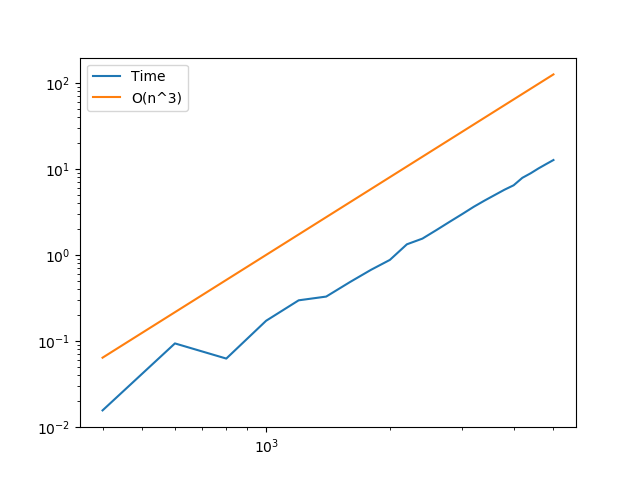
\includegraphics[width=\linewidth]{Aufgabe_1/plot_a.png}
    \caption{Rechenzeit abhängig von der Problemgröße}
    \label{fig:my_label}
\end{figure}
Wie in Abbildung 1 ersichtlich verhält sich die Rechenzeit kubisch in Relation zur Problemgröße.
Zum Testen wurde eine Zufallsmatrix mit 100 Nicht-Null-Einträgen pro Zeile (nicht exakt, da die Symmetriesierung den Wert pro
Zeile verzerrt) und einer Gesamtgröße von 500 erstellt. Der direkte Löser wurde schließlich auf die $(k200 \times k200)$-dimensionalen,
rechts oberen Untermatrizen angewandt ($2 \leq k \leq 25$).
\FloatBarrier
\subsection*{b)}
Implementierung des CG-Verfahrens:
\begin{lstlisting}[language=Python]
def cg(A,b,x0,tol):
    xt = x0
    r0 = b - np.dot(A,xt)
    d = r0
    count = 0
    while(np.linalg.norm(r0) > tol):
        prod = np.dot(np.transpose(r0),r0)
        prod2 = np.dot(A,d)
        alpha = prod/np.dot(np.transpose(d),prod2)
        xt = xt + alpha*d
        r0 = r0 - alpha*prod2
        beta = np.dot(np.transpose(r0),r0)/prod
        d = r0 + beta*d
        count += 1
    print(count)
    return xt
\end{lstlisting}
Beweis der Äquivalenz obigen Algorithmus zu Algorithmus 8.10 im Numerik-Skript:
